\documentclass{article}
\usepackage[utf8]{inputenc}
\usepackage{listings} % Uso de trechos de código no texto
\usepackage{indentfirst} % indentar primeiro parágrafo (desativado por padrão)
\usepackage{graphicx} % Uso de imagens
\usepackage[brazil]{babel} % Texto em português do Brasil
\usepackage{subfigure} % Uso de figuras no texto
\usepackage[a4paper, left=20mm, right=20mm, top=20mm, bottom=20mm]{geometry}
% Formatação da página: 20mm da margem

\begin{document}
\lstset{language=Prolog} % definindo o uso de trechos de código Prolog no texto.

\begin{center} 
    \section*{INE5416 - Paradigmas da Programação (2015/2)}
    \textbf{\textit{Projeto T3A: Processamento de imagens} \\
    Caique Rodrigues Marques 13204303 \\ 
    Gustavo José Carpeggiani 13103524 \\
    Vinícius Couto Biermann  13100778}
\end{center}

\section*{Regras}
    As seguintes regras foram implementadas na linguagem de programação SWI-Prolog, oferecendo operações a mais em relação à processamento de imagens. As imagens trabalhadas são em formato ascii pgm e em preto e branco, todas as implementações foram trabalhadas usando uma lista de pixels, que pode ser convertido para uma matriz de intensidade e vice-versa.
    
    \subsection*{negative}
        A regra faz com que, dada uma lista de pixels com intensidade I, seja retornado uma lista com as intensidades dos pixels sendo como 255-I, ou seja, ela faz com que as regiões mais claras das imagens fiquem mais escuras e as regiões mais escuras fiquem mais claras.

        A implementação em Prolog desta função, que está sendo mostrada abaixo em \textit{negative\_list/2}, funciona da seguinte forma: dada uma lista de entrada, a regra coleta a cabeça dela, ou seja, o primeiro elemento. A intensidade do pixel inicial da lista é alterado e adicionado à cabeça da lista de saída e o processo é novamente feito usando como entrada a cauda da lista de entrada, isto é, todos os elementos restantes, exceto o elemento inicial e a cauda da lista de saída, que armazenará o segundo elemento.

        O processo é realizado até a lista de entrada não conter mais elementos, neste caso, é adicionado nada ao final da lista de saída e a regra é interrompida (com o uso do sinal "!").

        \begin{lstlisting}[frame=single] % Início da região de uso de trecho de código.

        negative(FileName) :-
            atom_concat('imgs/', FileName, Path_file),
            print(Path_file), nl, nl,
            load(Path_file, C_list),
            negative_list(C_list, N_list),
            coord2matrix(N_list, Matrix),
            atom_string(FileName, String),
            atomic_list_concat(S_file, '.', String),
            nth0(0, S_file, Name),
            atom_concat(Name, '_negative.pgm', NewFileName),
            writePGM(NewFileName, Matrix),
            !.
            
        negative_list([], []) :- !.
        negative_list([(X, Y, I)|T_input], [H_output|T_output]) :-
            New_intensity is 255 - I,
            copy_term((X, Y, New_intensity), H_output),
            negative_list(T_input, T_output).    
        \end{lstlisting}
        
        Para testar a regra em uma imagem, \textit{negative/1} foi implementada. A imagem é especificada no parâmetro da regra e é retornado a imagem em negativo. Por exemplo, usando a imagem "\textit{lena.pgm}" é retornado o negativo como "\textit{lena\_negative.pgm}". A seguir, a imagem de entrada à esquerda e a imagem de saída à direita.
        
        \begin{figure}[h]
        \centering
            \begin{subfigure}
            \centering
            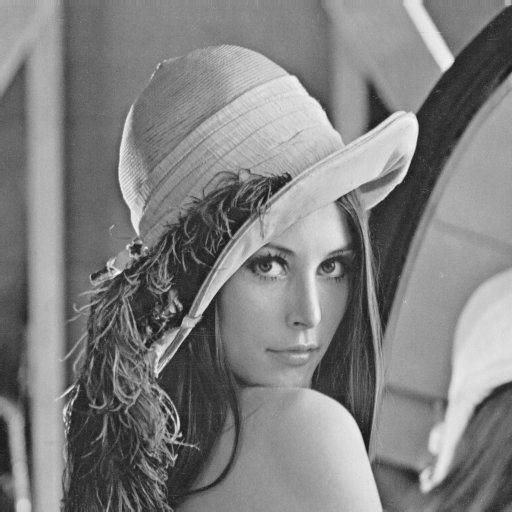
\includegraphics[width=139px, height=129px]{images/lena.jpg}
            \end{subfigure}
            \begin{subfigure}
            \centering
            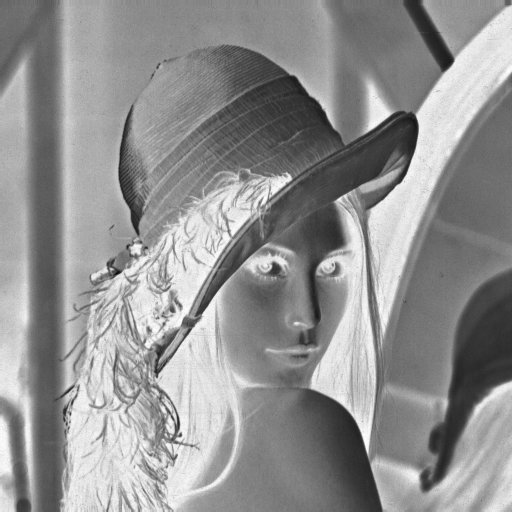
\includegraphics[width=139px, height=129px]{images/lena_negative.jpg}
            \end{subfigure}
        \end{figure}
        
    \newpage
    \subsection*{mean}
        Dadas duas imagens, a regra \textit{mean/2} define cada intensidade de um pixel da imagem resultante corresponde à soma das intensidades dos pixels correspondentes das duas imagens de mesmo tamanho divididos por dois, caso a divisão não seja exata, é arredondado para o valor mais próximo.

        A seguir, na regra \textit{mean\_list/3} é realizado a operação descrita acima. A regra recebe como parâmetro as duas listas a serem calculadas e a terceira lista é a lista de saída, as intensidades dos pixels correspondentes à respectiva imagem são adicionadas e divididos por dois, este novo ponto é armazenado na cabeça da lista. O funcionamento é semelhante ao da regra \textit{negative\_list/2}.
        
        \begin{lstlisting}[frame=single]
        mean(FileName1, FileName2) :-
            atom_concat('imgs/', FileName1, Path_f1),
            atom_concat('imgs/', FileName2, Path_f2),
            load(Path_f1, L1),
            load(Path_f2, L2),
            mean_list(L1, L2, L_output),
            coord2matrix(L_output, M_output),
        
            atom_string(FileName1, String1),
            atomic_list_concat(S_file1, '.', String1),
            nth0(0, S_file1, Name1),
        
            atom_string(FileName2, String2),
            atomic_list_concat(S_file2, '.', String2),
            nth0(0, S_file2, Name2),
        
            atom_concat(Name1, '_', T_name),
            atom_concat(T_name, Name2, Name_file),
            atom_concat(Name_file, '_mean.pgm', NewFileName),
            writePGM(NewFileName, M_output), !.
            
        mean_list([], [], []) :- !.
        mean_list([(X, Y, I1)|T1], [(_, _, I2)|T2], [H_output|T_output]) :-
            Mean_Intensity is (I1 + I2)/2,
            copy_term((X, Y, Mean_Intensity), H_output),
            mean_list(T1, T2, T_output).
        \end{lstlisting}
        
        A execução para gerar uma imagem com a média das intensidades é definido em \textit{mean/2}, que recebe como parâmetro duas imagens. Abaixo, um exemplo de média, com as imagens \textit{cameraman.pgm} e \textit{gull.pgm}, resultando em \textit{cameraman\_gull\_mean.pgm}.
    
        \begin{figure}[h]
        \centering
            \begin{subfigure}
            \centering
            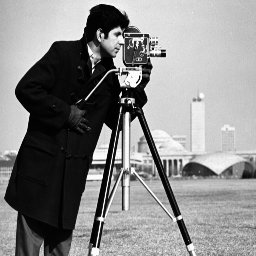
\includegraphics[width=139px, height=129px]{images/cameraman.jpg}
            \end{subfigure}
            \begin{subfigure}
            \centering
            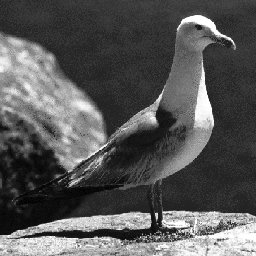
\includegraphics[width=139px, height=129px]{images/gull.jpg}
            \end{subfigure}
            \begin{subfigure}
            \centering
            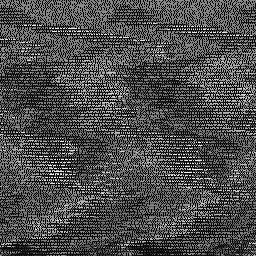
\includegraphics[width=139px, height=129px]{images/cameraman_gull_mean.jpg}
            \end{subfigure}
        \end{figure}    
        
    \newpage
    \subsection*{lonely\_pixel}
        Dado o pixel p1 de uma imagem, ele é dito isolado se todos os seus vizinhos (os pixels à esquerda, à direta, acima e abaixo) possuem as respectivas intensidades menores que a do pixel p1 em questão. A técnica pode ser usada para reconhecimento de imagens, como números escritos a mão.

        A regra abaixo implementa a técnica. Recebendo duas listas de pixels, uma para verificação dos vizinhos (\textit{C\_list}) e a outra como um contador, um acumulador (\textit{T\_acc}, a inicialização tem de ser uma lista vazia), para ir armazenando os pixels isolados, e uma lista de saída (\textit{Output}).
        
        O primeiro elemento da lista de contagem é usado como métrica inicial e os seus quatro vizinhos são encontrados graças à regra \textit{n4/3} e armazenado na lista \textit{Four\_list} (se o pixel estiver nas extremidades da imagem, pode retornar dois ou três vizinhos).
        
        A checagem da maior intensidade entre os quatro vizinhos é verificada na regra \textit{check\_n4\_intensity/2}, que recebe a lista com os quatro vizinhos e a intensidade de um pixel p1, onde em cada chamada, a regra verifica se os pixels da lista possuem intensidade menor que a intensidade de p1, definido em \textit{I\_base}.
        
        Se a checagem for verdadeira, ou seja, se o pixel p1 possui intensidade maior que os seus quatro vizinhos, então ele é considerado isolado e é adicionado à cabeça da lista de acumulador e a regra é chamada de novo com o próximo pixel da lista de contagem. Se a checagem for falsa, a regra é chamada novamente, com o acumulador intacto.

        Assim que todos os elementos da lista de contagem forem verificados, se a variável \textit{T\_acc} tiver pixels isolados, eles estarão em ordem do mais distante até o mais próximo do ponto de origem (0,0). É realizado uma inversão dos elementos da lista acumulador, com a regra nativa \textit{reverse/2}, e armazenado na lista de saída \textit{Output}.

        \begin{lstlisting}[frame=single]
        check_n4_intensity([], _) :- true, !.
        check_n4_intensity([(_, _, I)|Tail], I_base) :-
            I_base > I,
            check_n4_intensity(Tail, I_base).

        lonely_pixel(_, [], T_acc, Output) :-
            reverse(T_acc, Output).
        lonely_pixel(C_list, [(X, Y, I)|Tail], T_acc, Output) :-
            n4(C_list, (X, Y, I), Four_list),
            (
                check_n4_intensity(Four_list, I) ->
                    lonely_pixel(C_list, Tail, [(X, Y, I)|T_acc], Output);
                lonely_pixel(C_list, Tail, T_acc, Output)
            ).
        \end{lstlisting}

        A seguir, um exemplo usando uma matriz de intensidades, onde as linhas e as colunas estão especificados acima e à direita da matriz, respectivamente. Após a execução de um teste desta regra na matriz, o resultado é uma lista com os pixels isolados.

        \begin{verbatim}
 0,1,2,3,4,5,6,7,8,9
[4,0,0,0,0,0,0,0,0,0] 0
[1,1,0,0,1,9,0,0,0,0] 1
[0,1,0,0,1,0,0,0,0,0] 2
[0,0,0,0,0,0,0,0,0,0] 3
[0,0,3,0,0,0,1,0,0,0] 4
[0,7,1,0,0,0,0,0,0,0] 5
[0,0,0,0,0,0,0,5,1,0] 6
[0,0,0,0,0,0,0,0,0,0] 7
[0,0,0,0,0,0,0,0,0,0] 8
[0,0,0,0,0,0,0,0,0,0] 9

?- test_lonely_pixel.
[ (0,0,4), (1,5,9), (4,2,3), (4,6,1), (5,1,7), (6,7,5)]
true.

        \end{verbatim}

    \newpage
    \subsection*{path\_pixels}
        Dados dois pixels, há um caminho entre eles se o conjunto dos pixels adjacentes (considerando os quatro vizinhos, ou seja, os pixels à esquerda, à direita, acima e abaixo do pixel em questão) que pode alcançar ao pixel final. Portanto, para o camanho, os pixels possuem intensidades maiores ou iguais à intensidade do pixel inicial.
        
        A regra, mostrada abaixo, recebe uma lista com todos os pixels, o pixel inicial, o pixel destino, um acumulador (sua inicialização tem de ser uma lista vazia) e usará uma segunda lista com o caminho realizado. Primeiramente, as intensidades dos pixels inicial e destino são encontrados.
        
        Uma condição é checada e será explicada posteriormente, se ela retornar falso, os quatro vizinhos do pixel inicial são encontrados e armazenados em \textit{Four\_list}. Duas regras nativas são usadas para remover possíveis redundâncias em \textit{Four\_list}, ou seja, pontos que já foram passados, evitando loops infinitos; a regra \textit{intersection/3} coloca a interseção dos elementos das duas listas em \textit{Intersection}, que possui os elementos em comum, depois, os elementos desta lista são os mesmos removidos de \textit{Four\_list} e os restantes são adicionados ao \textit{New\_4list}, assim sendo, os elementos que já foram marcados, não são referenciados novamente.
        
        Depois, a regra \textit{get\_bigger\_intensity/3} é chamada enviando a lista e o pixel inicial, nesta regra é checado qual o pixel com intensidade maior ou igual ao inicial, a resposta disto é armazenada no final em \textit{Bigger}.
        
        Mais uma condição é checada, se o pixel \textit{Bigger} é igual a algum elemento da lista de saída, se sim, isto significa que não houve movimentação, ou seja, o pixel inicial possui vizinhos com intensidades menores do que a sua, impossibilitando um caminho. Caso contrário, a regra \textit{path\_pixels/4} é chamada novamente. Na segunda iteração é recebido a lista com todos os pixels, o pixel inicial é adicionado à cabeça do acumulador e novo pixel base é o \textit{Bigger}.
        
        Todo o processo é repetido até cair na condição \textit{check\_destiny/2}, onde verificará se o pixel inicial é igual ao pixel destino, se sim, significa que existe um caminho e a regra termina, se não, continua o código, que já foi explicado antes.
        \begin{lstlisting}[frame=single]
path_pixels([], _, _, T_acc, Output) :- reverse(T_acc, Output).
path_pixels(C_list, (Xs, Ys, _), (Xd, Yd, _), T_acc, Output) :-
    getPixel(C_list, (Xs, Ys, Is)),
    getPixel(C_list, (Xd, Yd, Id)),
    (
        check_destiny((Xs, Ys, Is), (Xd, Yd, Id)) ->
            writeln('Path found!'),
            reverse([(Xs, Ys, Is)|T_acc], Output),
            true;
        n4(C_list, (Xs, Ys, Is), Four_list),
        intersection(Four_list, T_acc, Intersection),
        subtract(Four_list, Intersection, New_4list),
        get_bigger_intensity(New_4list, (Xs, Ys, Is), Bigger),
        (
            check_loop(T_acc, Bigger) ->
                writeln('Path not found.'),
                reverse([(Xs, Ys, Is)|T_acc], Output);
            path_pixels(C_list, Bigger, (Xd, Yd, Id), 
                        [(Xs, Ys, Is)|T_acc], Output)
        )
    ).
        \end{lstlisting}
        
        Após a execução da regra é possível ver o caminho percorrido do pixel inicial até o pixel destino, se este caminho não existir, ainda assim é possível ver até onde o pixel alcançou, bastando usar o comando \textit{print/1} com a lista de saída. A seguir, dois testes usando a imagem \textit{ufsc.pgm}.

        \begin{verbatim}
?- test_path_pixels((0,0,_),(5,1,_)).
Path found!
[ (0,0,0), (0,1,0), (1,1,50), (2,1,50), (3,1,50), (4,1,50), (5,1,50)]
true.

?- test_path_pixels((0, 0, _), (3,7, _)).
Path not found.
[ (0,0,0), (0,1,0), (1,1,50), (2,1,50), (3,1,50), (4,1,50), (5,1,50), (5,2,50),
(5,3,50), (5,4,50), (4,4,50), (3,4,50), (2,4,50), (1,4,50), (1,4,50)]
    \end{verbatim}

    \newpage
    \subsection*{dark\_pixels e clear\_pixels}
        As imagens usadas para este projeto são em preto e branco, portanto, o esquema de cores é de 256 cores, quando a intensidade estiver mais próxima do zero, a tonalidade da cor tende a ser mais escura até o preto, enquanto intensidade mais próxima de 255, a tonalidade da cor tende a ser mais clara até o branco. As regras \textit{dark\_pixels} e \textit{clear\_pixels} coletam os pixels mais escuros e claros de uma imagem, respectivamente, e o intensificam, de forma que fiquem mais evidentes.
        
        As duas regras usam uma outra para coletar os pixels, \textit{get\_dark\_pixels\_image} e \textit{get\_clear\_pixels\_image}, que verifica a intensidade de cada pixel e, se a condição imposta não for satisfeita, o pixel é armazenado na lista de saída. Caso contrário, a intensidade é aumentada ou diminuída de forma que na imagem resultante fique evidente as regiões mais claras e escuras de uma imagem.
        
        Mais duas regras semelhantes a estas foram implementadas com a terminação \textit{list} tal que, ao invés de aumentar ou diminuir a tonalidade, a lista de saída está apenas com os pixels desejados, sem modificar a intensidade.
        \begin{lstlisting}[frame=single]
    dark_pixels(FileName) :-
        atom_concat('imgs/', FileName, Path_file),
        print(Path_file), nl, nl,
        load(Path_file, C_list),
        get_dark_pixels_image(C_list, [], Dark_list),
        coord2matrix(Dark_list, Matrix),
        atom_string(FileName, String),
        atomic_list_concat(S_file, '.', String),
        nth0(0, S_file, Name),
        atom_concat(Name, '_dark.pgm', NewFileName),
        writePGM(NewFileName, Matrix), !.
    
    get_clear_pixels_image([], T_acc, Dark_list) :-
        reverse(T_acc, Dark_list).
    get_clear_pixels_image([(X, Y, I)|T_input], T_acc, Dark_list) :-
        (
            I > 127 ->
                get_clear_pixels_image(T_input, [(X,Y,255)|T_acc], Dark_list);
            get_clear_pixels_image(T_input, [(X,Y,I)|T_acc], Dark_list)
        ).
        
    get_dark_pixels_list([], T_acc, Dark_list) :-
        reverse(T_acc, Dark_list).
    get_dark_pixels_list([(X, Y, I)|T_input], T_acc, Dark_list) :-
        (
            I =< 127 ->
                get_dark_pixels_list(T_input, [(X,Y,I)|T_acc], Dark_list);
            get_dark_pixels_list(T_input, T_acc, Dark_list)
        ).
        \end{lstlisting}

        A seguir a execução das regras com a imagem \textit{lena.pgm}, resultando em \textit{lena\_dark.pgm} e \textit{lena\_clear.pgm}, nesta ordem da esquerda para a direita.
        \begin{figure}[h]
        \centering
            \begin{subfigure}
            \centering
            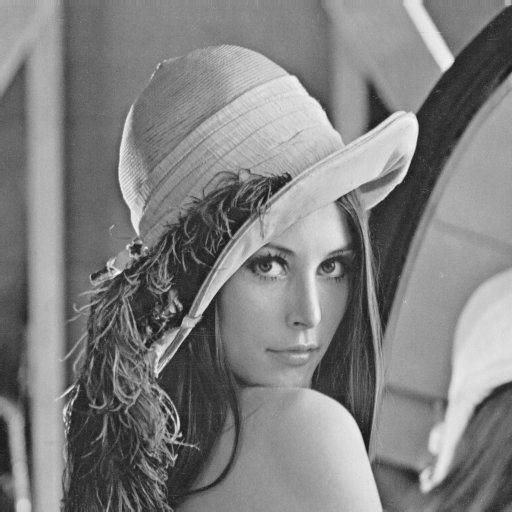
\includegraphics[width=139px, height=129px]{images/lena.jpg}
            \end{subfigure}
            \begin{subfigure}
            \centering
            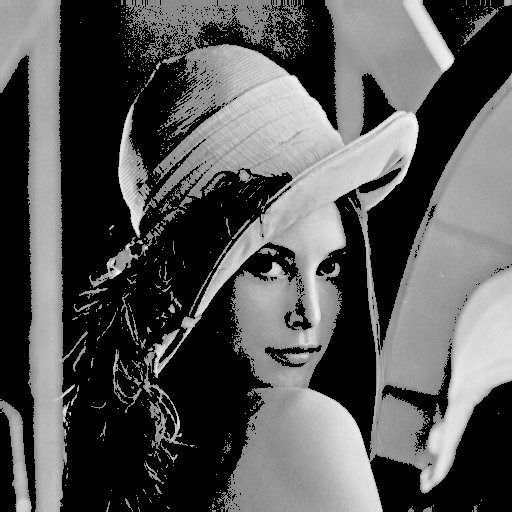
\includegraphics[width=139px, height=129px]{images/lena_dark.jpg}
            \end{subfigure}
            \begin{subfigure}
            \centering
            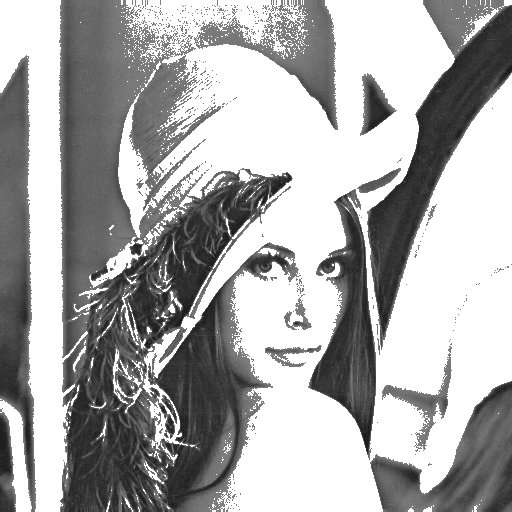
\includegraphics[width=139px, height=129px]{images/lena_clear.jpg}
            \end{subfigure}
        \end{figure}

\end{document}
